%=====================================================================
%  IC PROJECT SYNOPSIS -- LectureAssist
%  Compile on Overleaf with pdfLaTeX. Single file, no uploads needed.
%
%  FONT: the template requires Calibri 10pt. Calibri is proprietary and
%  is NOT installed on Overleaf, so this file uses Carlito -- the
%  metric-compatible open clone of Calibri (identical widths, so the
%  page fills exactly as Calibri would). For literal Calibri: upload
%  calibri.ttf / calibrib.ttf / calibrii.ttf / calibriz.ttf, switch the
%  compiler to XeLaTeX, delete the fontenc + inputenc + carlito lines
%  below and replace them with:
%     \usepackage{fontspec}
%     \setmainfont{calibri.ttf}[BoldFont=calibrib.ttf,
%       ItalicFont=calibrii.ttf,BoldItalicFont=calibriz.ttf]
%
%  FIGURE: drawn inline with TikZ -- metho.svg is NOT used here. The
%  book's vertical diagram is far too tall for a synopsis, so this is a
%  wide two-row version of the same pipeline, spanning both columns.
%  Nothing to upload.
%
%  WORD COUNTS (checked against the template limits):
%     Abstract        98 / 100
%     Method         100 / 100
%     Novelty         50 / 50
%     Impact          50 / 50
%     Business Model  95 / 100
%     Conclusion      50 / 50
%=====================================================================

\documentclass[10pt,a4paper]{article}

\usepackage[T1]{fontenc}
\usepackage[utf8]{inputenc}
\usepackage[sfdefault]{carlito}   % metric-compatible Calibri clone
\usepackage[margin=0.9in]{geometry}
\usepackage{multicol}
\usepackage{graphicx}
\usepackage{caption}
\usepackage{parskip}
\usepackage{needspace}
\usepackage{tikz}
\usetikzlibrary{positioning,arrows.meta,fit,backgrounds,calc}

\setlength{\columnsep}{20pt}
\raggedcolumns   % stop multicol stretching blank space to balance columns
\captionsetup{font=small,labelfont=bf,justification=raggedright,
              singlelinecheck=false}
\pagestyle{empty}

% Section heading in the template's style: bold, run-in, tight spacing.
% \needspace stops a heading being stranded alone at a column foot.
\newcommand{\synsection}[1]{%
  \needspace{3\baselineskip}%
  \vspace{0.55em}\noindent\textbf{#1}\par\vspace{0.25em}}

% ---- diagram palette -------------------------------------------------
% Two colour families encode the two pipeline stages; one muted red is
% reserved exclusively for the failure/retry path. Nothing is coloured
% decoratively -- colour always carries meaning.
\definecolor{stageA}{HTML}{1B4F72}   % ingestion / representation
\definecolor{stageB}{HTML}{7E5109}   % agentic generation
\definecolor{failc} {HTML}{922B21}   % failure + retry path only
\definecolor{inkgy} {HTML}{4D4D4D}

% node text: bold coloured agent name over a lighter grey descriptor
\newcommand{\nt}[1]{{\hyphenpenalty=10000\exhyphenpenalty=10000
  \fontsize{7.0}{7.9}\selectfont\bfseries #1}}
\newcommand{\nd}[1]{{\hyphenpenalty=10000\exhyphenpenalty=10000
  \fontsize{6.3}{7.2}\selectfont\color{inkgy}#1}}

% ---- diagram styles --------------------------------------------------
\tikzset{
  % an AGENT: white ground, coloured hairline -- something that acts
  agent/.style  = {draw=#1!60, line width=0.5pt, fill=white,
                   rounded corners=1.2pt, align=flush center,
                   minimum height=12mm, text width=28mm, inner sep=2.5pt},
  agent/.default = stageA,
  % a DATA ARTIFACT: tinted ground, no hard edge -- something that is
  data/.style   = {draw=#1!25, line width=0.4pt, fill=#1!7,
                   rounded corners=1.2pt, align=flush center,
                   minimum height=12mm, text width=28mm, inner sep=2.5pt},
  data/.default  = stageA,
  band/.style   = {rounded corners=2.5pt, draw=none, fill=#1!5},
  band/.default = stageA,
  flow/.style   = {-{Latex[length=1.5mm,width=1.3mm]}, draw=#1!75,
                   line width=0.5pt, rounded corners=1.5pt},
  flow/.default = stageA,
  retry/.style  = {-{Latex[length=1.5mm,width=1.3mm]}, draw=failc,
                   line width=0.5pt, dash pattern=on 1.1mm off 0.7mm,
                   rounded corners=2pt},
  elbl/.style   = {fill=white, inner sep=1.5pt,
                   font=\fontsize{6.0}{6.8}\selectfont},
  stage/.style  = {font=\fontsize{6.2}{7}\selectfont\bfseries,
                   text=#1, inner sep=0pt},
  stage/.default = stageA,
}

\begin{document}

%---------------------------------------------------------------
% TITLE BLOCK (spans both columns)
%---------------------------------------------------------------
\begin{center}
  {\bfseries LectureAssist: An Agentic Multimodal AI Assistant that Turns
   Lectures into Adaptive Study Material}\\[0.3em]
  Fully local, zero-paid-API question generation from lecture video and
  course documents\\[0.5em]
  % Delete the next two lines if the department wants an anonymous synopsis.
  {\small Iftikhar Ahmed (2121019642) \quad Salman Shafi (2211386042)
   \quad Jarinah Tasnim (2121026642)}\\
  {\small Supervisor: Dr.\ Adnan Areefen, Department of Electrical and
   Computer Engineering, North South University}
\end{center}

\vspace{0.6em}

\begin{multicols}{2}

%---------------------------------------------------------------
% ABSTRACT -- 98 words
%---------------------------------------------------------------
\synsection{ABSTRACT}

Lecture recordings and course documents are everywhere, but the tools
that turn them into real practice are not. Most study aids expect clean
text pasted in by hand, or run on paid cloud APIs that few students can
afford. LectureAssist takes a raw lecture video or a document and
produces study and assessment material on its own, with no paid service
anywhere. It reads the board and the slides with OCR, listens to the
audio with Whisper, and then a team of agents plans, retrieves, writes,
checks and rewrites quiz questions. Chat and adaptive difficulty close
the loop.

%---------------------------------------------------------------
% METHOD -- 100 words
%---------------------------------------------------------------
\synsection{Method with System Diagram/Design Complexity}

An orchestrator coordinates specialist agents. Video is sampled into
frames and audio demuxed; documents are parsed directly. Each frame is
classified by brightness and edge statistics as slide, blackboard,
whiteboard or scene, then preprocessed before OCR; Faster-Whisper
transcribes speech. Both channels fuse into one timestamped timeline,
then summarised, chunked, embedded and indexed in FAISS. A Quiz Planner
allocates topic-difficulty slots; a Generator drafts one question at a
time, invoking retrieval as a tool when context is insufficient; a
Validator returns PASS or FAIL with a remediation action; a Refiner
retries within budget. Models are Gemma~3, served locally by Ollama.

\end{multicols}

%---------------------------------------------------------------
% THE ONE DIAGRAM ALLOWED BY THE TEMPLATE -- spans both columns.
% Drawn in draw.io (Book/synopsis-architecture.drawio) and exported to PDF.
% PDF rather than SVG on purpose: draw.io exports HTML labels as
% <foreignObject>, which Inkscape (used by the svg package) does not render,
% so an SVG here would silently lose every caption.
%---------------------------------------------------------------
\begin{center}
  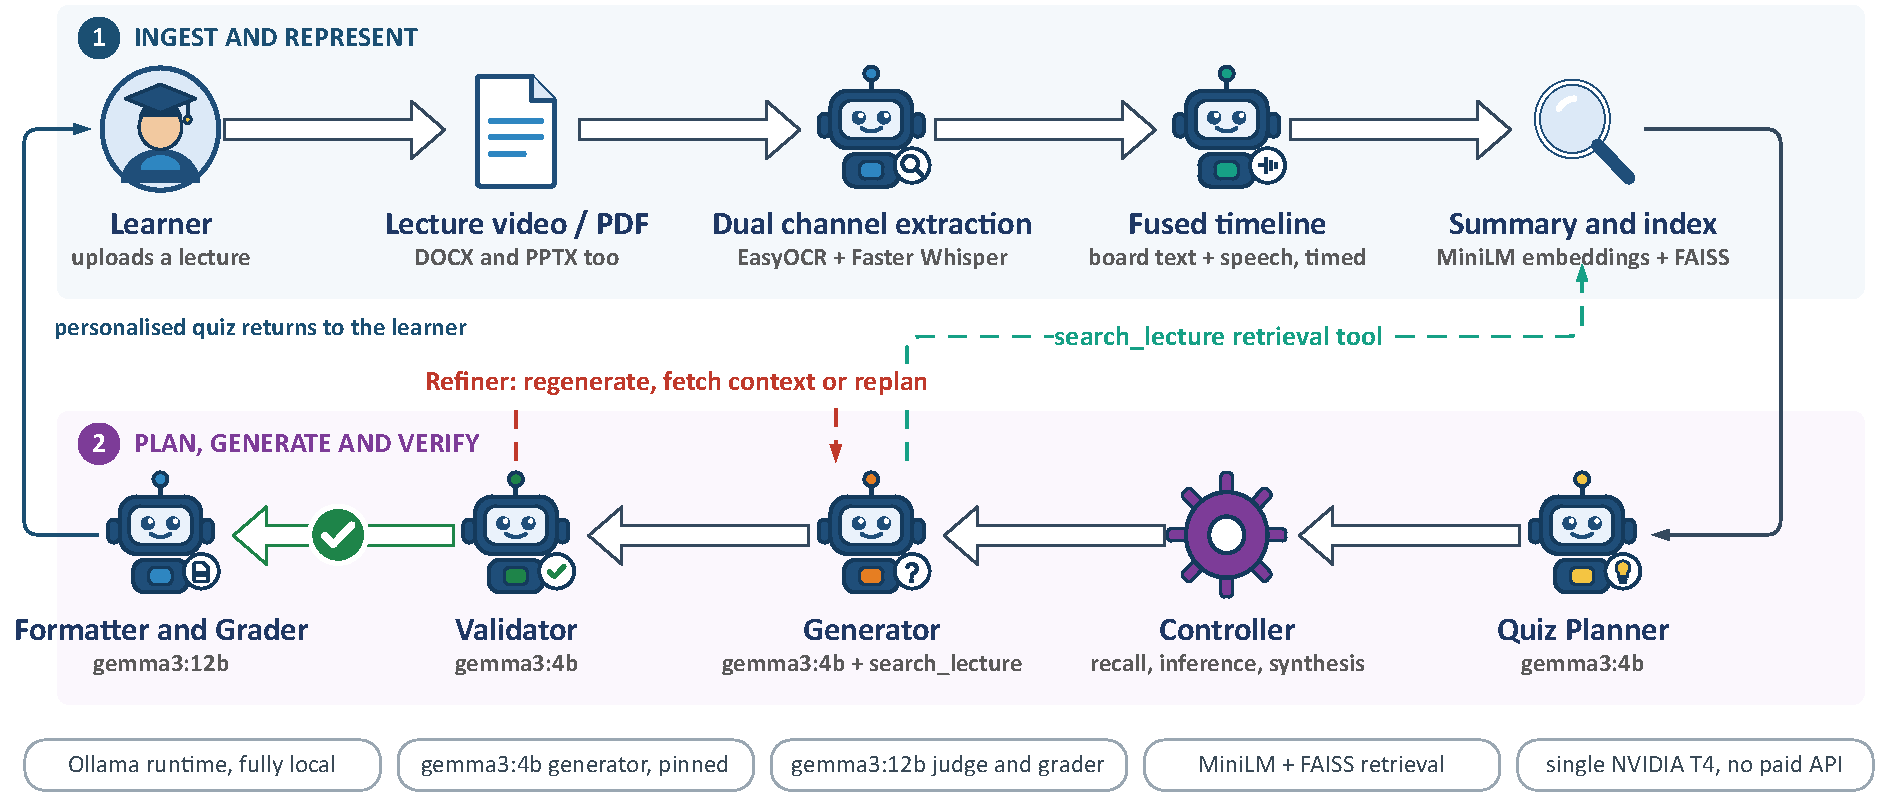
\includegraphics[width=\textwidth]{synopsis-architecture.pdf}
\end{center}
\vspace{-0.8em}
\captionof{figure}{LectureAssist architecture. Row~1 turns raw media into
one grounded representation; row~2 is the agentic loop, where a failed
question is diagnosed and routed back for regeneration, not discarded.}
\vspace{0.4em}

\begin{multicols}{2}

%---------------------------------------------------------------
% NOVELTY -- 50 words
%---------------------------------------------------------------
\synsection{Novelty of Project}

Two elements are new. Extraction is scene-adaptive rather than a single
OCR recipe, so handwritten board work and projected slides survive. And
the validator diagnoses a failed question, choosing whether to
regenerate, fetch context or replan the topic, instead of merely
filtering. Comparable tools need pasted text or paid APIs.

%---------------------------------------------------------------
% IMPACT -- 50 words
%---------------------------------------------------------------
\synsection{Impact on Society/Environment}

Retrieval practice is a highly effective study strategy, but good
practice questions are unevenly distributed. Generating them from a
student's own lectures, on hardware they already own, removes a cost
barrier rather than an ability barrier, supporting SDG~4 and~10. Local
4B inference also avoids datacentre-scale energy per query.

%---------------------------------------------------------------
% BUSINESS MODEL -- 95 words
%---------------------------------------------------------------
\synsection{Business Model/Feasibility/Financial Scalability Plan}

Marginal cost per student is near zero: no paid API is used, and the
only input is compute the user already owns. The plan is a free,
open-source self-hosted tier for individual students, and a paid
institutional tier in which a department runs one GPU server for an
entire course, licensed per seat per semester at a fraction of
per-token cloud pricing. Revenue comes from institutional licences, LMS
integration and support rather than student subscriptions. Feasibility
is already demonstrated: the whole system runs on a free-tier T4, so one
modest GPU can serve a class.

%---------------------------------------------------------------
% CONCLUSION -- 50 words
%---------------------------------------------------------------
\synsection{Conclusion}

The pipeline, extraction, retrieval, generation, grading and adaptation,
is implemented and running. Two of four generation pipelines have
completed a scored run of 200 MCQs each; on native metrics the
non-agentic baseline currently matches or beats the agentic loop, which
duplicates more. EQGBench and ReQUESTA harnesses are built but unrun.

\end{multicols}

\end{document}



